% Created by tikzDevice version 0.12 on 2018-10-15 11:51:21
% !TEX encoding = UTF-8 Unicode
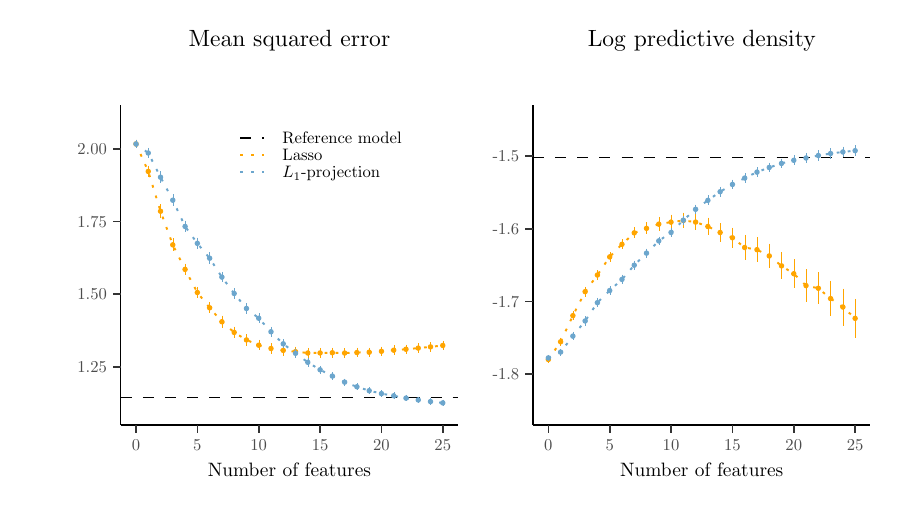
\begin{tikzpicture}[x=1pt,y=1pt]
\definecolor{fillColor}{RGB}{255,255,255}
\path[use as bounding box,fill=fillColor,fill opacity=0.00] (0,0) rectangle (310.76,166.22);
\begin{scope}
\path[clip] (  0.00,140.34) rectangle (161.76,166.22);
\definecolor{drawColor}{RGB}{255,255,255}
\definecolor{fillColor}{RGB}{255,255,255}

\path[draw=drawColor,line width= 0.6pt,line join=round,line cap=round,fill=fillColor] ( -0.00,140.34) rectangle (161.76,166.22);
\end{scope}
\begin{scope}
\path[clip] (  0.00,  0.00) rectangle (161.76,140.34);
\definecolor{drawColor}{RGB}{255,255,255}
\definecolor{fillColor}{RGB}{255,255,255}

\path[draw=drawColor,line width= 0.6pt,line join=round,line cap=round,fill=fillColor] ( -0.00,  0.00) rectangle (161.76,140.34);
\end{scope}
\begin{scope}
\path[clip] (161.76,140.34) rectangle (310.76,166.22);
\definecolor{drawColor}{RGB}{255,255,255}
\definecolor{fillColor}{RGB}{255,255,255}

\path[draw=drawColor,line width= 0.6pt,line join=round,line cap=round,fill=fillColor] (161.76,140.34) rectangle (310.76,166.22);
\end{scope}
\begin{scope}
\path[clip] (161.76,  0.00) rectangle (310.76,140.34);
\definecolor{drawColor}{RGB}{255,255,255}
\definecolor{fillColor}{RGB}{255,255,255}

\path[draw=drawColor,line width= 0.6pt,line join=round,line cap=round,fill=fillColor] (161.76,  0.00) rectangle (310.76,140.34);
\end{scope}
\begin{scope}
\path[clip] ( 33.59,143.09) rectangle (155.55,166.22);
\definecolor{drawColor}{RGB}{0,0,0}

\node[text=drawColor,anchor=base,inner sep=0pt, outer sep=0pt, scale=  0.85] at ( 94.57,159.29) {Mean squared error};
\end{scope}
\begin{scope}
\path[clip] ( 33.59, 22.62) rectangle (155.55,138.26);
\definecolor{fillColor}{RGB}{255,255,255}

\path[fill=fillColor] ( 33.59, 22.62) rectangle (155.55,138.26);
\definecolor{drawColor}{RGB}{0,0,0}

\path[draw=drawColor,line width= 0.3pt,dash pattern=on 4pt off 4pt ,line join=round] ( 33.59, 32.72) -- (155.55, 32.72);
\definecolor{drawColor}{RGB}{255,165,0}

\path[draw=drawColor,line width= 0.7pt,dash pattern=on 1pt off 3pt ,line join=round] ( 39.14,124.20) --
	( 43.57,114.27) --
	( 48.01, 99.88) --
	( 52.44, 87.74) --
	( 56.88, 78.87) --
	( 61.31, 70.52) --
	( 65.75, 65.01) --
	( 70.18, 59.96) --
	( 74.62, 56.10) --
	( 79.05, 53.39) --
	( 83.48, 51.49) --
	( 87.92, 50.29) --
	( 92.35, 49.60) --
	( 96.79, 49.14) --
	(101.22, 48.67) --
	(105.66, 48.69) --
	(110.09, 48.77) --
	(114.53, 48.65) --
	(118.96, 48.82) --
	(123.40, 48.95) --
	(127.83, 49.27) --
	(132.27, 49.68) --
	(136.70, 50.02) --
	(141.13, 50.43) --
	(145.57, 50.88) --
	(150.00, 51.38);
\definecolor{fillColor}{RGB}{255,165,0}

\path[draw=drawColor,line width= 0.4pt,line join=round,line cap=round,fill=fillColor] ( 39.14,124.20) circle (  0.78);

\path[draw=drawColor,line width= 0.4pt,line join=round,line cap=round,fill=fillColor] ( 43.57,114.27) circle (  0.78);

\path[draw=drawColor,line width= 0.4pt,line join=round,line cap=round,fill=fillColor] ( 48.01, 99.88) circle (  0.78);

\path[draw=drawColor,line width= 0.4pt,line join=round,line cap=round,fill=fillColor] ( 52.44, 87.74) circle (  0.78);

\path[draw=drawColor,line width= 0.4pt,line join=round,line cap=round,fill=fillColor] ( 56.88, 78.87) circle (  0.78);

\path[draw=drawColor,line width= 0.4pt,line join=round,line cap=round,fill=fillColor] ( 61.31, 70.52) circle (  0.78);

\path[draw=drawColor,line width= 0.4pt,line join=round,line cap=round,fill=fillColor] ( 65.75, 65.01) circle (  0.78);

\path[draw=drawColor,line width= 0.4pt,line join=round,line cap=round,fill=fillColor] ( 70.18, 59.96) circle (  0.78);

\path[draw=drawColor,line width= 0.4pt,line join=round,line cap=round,fill=fillColor] ( 74.62, 56.10) circle (  0.78);

\path[draw=drawColor,line width= 0.4pt,line join=round,line cap=round,fill=fillColor] ( 79.05, 53.39) circle (  0.78);

\path[draw=drawColor,line width= 0.4pt,line join=round,line cap=round,fill=fillColor] ( 83.48, 51.49) circle (  0.78);

\path[draw=drawColor,line width= 0.4pt,line join=round,line cap=round,fill=fillColor] ( 87.92, 50.29) circle (  0.78);

\path[draw=drawColor,line width= 0.4pt,line join=round,line cap=round,fill=fillColor] ( 92.35, 49.60) circle (  0.78);

\path[draw=drawColor,line width= 0.4pt,line join=round,line cap=round,fill=fillColor] ( 96.79, 49.14) circle (  0.78);

\path[draw=drawColor,line width= 0.4pt,line join=round,line cap=round,fill=fillColor] (101.22, 48.67) circle (  0.78);

\path[draw=drawColor,line width= 0.4pt,line join=round,line cap=round,fill=fillColor] (105.66, 48.69) circle (  0.78);

\path[draw=drawColor,line width= 0.4pt,line join=round,line cap=round,fill=fillColor] (110.09, 48.77) circle (  0.78);

\path[draw=drawColor,line width= 0.4pt,line join=round,line cap=round,fill=fillColor] (114.53, 48.65) circle (  0.78);

\path[draw=drawColor,line width= 0.4pt,line join=round,line cap=round,fill=fillColor] (118.96, 48.82) circle (  0.78);

\path[draw=drawColor,line width= 0.4pt,line join=round,line cap=round,fill=fillColor] (123.40, 48.95) circle (  0.78);

\path[draw=drawColor,line width= 0.4pt,line join=round,line cap=round,fill=fillColor] (127.83, 49.27) circle (  0.78);

\path[draw=drawColor,line width= 0.4pt,line join=round,line cap=round,fill=fillColor] (132.27, 49.68) circle (  0.78);

\path[draw=drawColor,line width= 0.4pt,line join=round,line cap=round,fill=fillColor] (136.70, 50.02) circle (  0.78);

\path[draw=drawColor,line width= 0.4pt,line join=round,line cap=round,fill=fillColor] (141.13, 50.43) circle (  0.78);

\path[draw=drawColor,line width= 0.4pt,line join=round,line cap=round,fill=fillColor] (145.57, 50.88) circle (  0.78);

\path[draw=drawColor,line width= 0.4pt,line join=round,line cap=round,fill=fillColor] (150.00, 51.38) circle (  0.78);

\path[draw=drawColor,line width= 0.1pt,line join=round] ( 39.14,125.75) --
	( 39.14,125.75);

\path[draw=drawColor,line width= 0.1pt,line join=round] ( 39.14,125.75) --
	( 39.14,122.64);

\path[draw=drawColor,line width= 0.1pt,line join=round] ( 39.14,122.64) --
	( 39.14,122.64);

\path[draw=drawColor,line width= 0.1pt,line join=round] ( 43.57,116.41) --
	( 43.57,116.41);

\path[draw=drawColor,line width= 0.1pt,line join=round] ( 43.57,116.41) --
	( 43.57,112.13);

\path[draw=drawColor,line width= 0.1pt,line join=round] ( 43.57,112.13) --
	( 43.57,112.13);

\path[draw=drawColor,line width= 0.1pt,line join=round] ( 48.01,102.38) --
	( 48.01,102.38);

\path[draw=drawColor,line width= 0.1pt,line join=round] ( 48.01,102.38) --
	( 48.01, 97.39);

\path[draw=drawColor,line width= 0.1pt,line join=round] ( 48.01, 97.39) --
	( 48.01, 97.39);

\path[draw=drawColor,line width= 0.1pt,line join=round] ( 52.44, 90.06) --
	( 52.44, 90.06);

\path[draw=drawColor,line width= 0.1pt,line join=round] ( 52.44, 90.06) --
	( 52.44, 85.42);

\path[draw=drawColor,line width= 0.1pt,line join=round] ( 52.44, 85.42) --
	( 52.44, 85.42);

\path[draw=drawColor,line width= 0.1pt,line join=round] ( 56.88, 80.97) --
	( 56.88, 80.97);

\path[draw=drawColor,line width= 0.1pt,line join=round] ( 56.88, 80.97) --
	( 56.88, 76.77);

\path[draw=drawColor,line width= 0.1pt,line join=round] ( 56.88, 76.77) --
	( 56.88, 76.77);

\path[draw=drawColor,line width= 0.1pt,line join=round] ( 61.31, 72.58) --
	( 61.31, 72.58);

\path[draw=drawColor,line width= 0.1pt,line join=round] ( 61.31, 72.58) --
	( 61.31, 68.47);

\path[draw=drawColor,line width= 0.1pt,line join=round] ( 61.31, 68.47) --
	( 61.31, 68.47);

\path[draw=drawColor,line width= 0.1pt,line join=round] ( 65.75, 67.08) --
	( 65.75, 67.08);

\path[draw=drawColor,line width= 0.1pt,line join=round] ( 65.75, 67.08) --
	( 65.75, 62.94);

\path[draw=drawColor,line width= 0.1pt,line join=round] ( 65.75, 62.94) --
	( 65.75, 62.94);

\path[draw=drawColor,line width= 0.1pt,line join=round] ( 70.18, 62.14) --
	( 70.18, 62.14);

\path[draw=drawColor,line width= 0.1pt,line join=round] ( 70.18, 62.14) --
	( 70.18, 57.78);

\path[draw=drawColor,line width= 0.1pt,line join=round] ( 70.18, 57.78) --
	( 70.18, 57.78);

\path[draw=drawColor,line width= 0.1pt,line join=round] ( 74.62, 58.23) --
	( 74.62, 58.23);

\path[draw=drawColor,line width= 0.1pt,line join=round] ( 74.62, 58.23) --
	( 74.62, 53.98);

\path[draw=drawColor,line width= 0.1pt,line join=round] ( 74.62, 53.98) --
	( 74.62, 53.98);

\path[draw=drawColor,line width= 0.1pt,line join=round] ( 79.05, 55.43) --
	( 79.05, 55.43);

\path[draw=drawColor,line width= 0.1pt,line join=round] ( 79.05, 55.43) --
	( 79.05, 51.34);

\path[draw=drawColor,line width= 0.1pt,line join=round] ( 79.05, 51.34) --
	( 79.05, 51.34);

\path[draw=drawColor,line width= 0.1pt,line join=round] ( 83.48, 53.42) --
	( 83.48, 53.42);

\path[draw=drawColor,line width= 0.1pt,line join=round] ( 83.48, 53.42) --
	( 83.48, 49.57);

\path[draw=drawColor,line width= 0.1pt,line join=round] ( 83.48, 49.57) --
	( 83.48, 49.57);

\path[draw=drawColor,line width= 0.1pt,line join=round] ( 87.92, 52.23) --
	( 87.92, 52.23);

\path[draw=drawColor,line width= 0.1pt,line join=round] ( 87.92, 52.23) --
	( 87.92, 48.36);

\path[draw=drawColor,line width= 0.1pt,line join=round] ( 87.92, 48.36) --
	( 87.92, 48.36);

\path[draw=drawColor,line width= 0.1pt,line join=round] ( 92.35, 51.46) --
	( 92.35, 51.46);

\path[draw=drawColor,line width= 0.1pt,line join=round] ( 92.35, 51.46) --
	( 92.35, 47.73);

\path[draw=drawColor,line width= 0.1pt,line join=round] ( 92.35, 47.73) --
	( 92.35, 47.73);

\path[draw=drawColor,line width= 0.1pt,line join=round] ( 96.79, 50.97) --
	( 96.79, 50.97);

\path[draw=drawColor,line width= 0.1pt,line join=round] ( 96.79, 50.97) --
	( 96.79, 47.30);

\path[draw=drawColor,line width= 0.1pt,line join=round] ( 96.79, 47.30) --
	( 96.79, 47.30);

\path[draw=drawColor,line width= 0.1pt,line join=round] (101.22, 50.49) --
	(101.22, 50.49);

\path[draw=drawColor,line width= 0.1pt,line join=round] (101.22, 50.49) --
	(101.22, 46.85);

\path[draw=drawColor,line width= 0.1pt,line join=round] (101.22, 46.85) --
	(101.22, 46.85);

\path[draw=drawColor,line width= 0.1pt,line join=round] (105.66, 50.49) --
	(105.66, 50.49);

\path[draw=drawColor,line width= 0.1pt,line join=round] (105.66, 50.49) --
	(105.66, 46.90);

\path[draw=drawColor,line width= 0.1pt,line join=round] (105.66, 46.90) --
	(105.66, 46.90);

\path[draw=drawColor,line width= 0.1pt,line join=round] (110.09, 50.57) --
	(110.09, 50.57);

\path[draw=drawColor,line width= 0.1pt,line join=round] (110.09, 50.57) --
	(110.09, 46.98);

\path[draw=drawColor,line width= 0.1pt,line join=round] (110.09, 46.98) --
	(110.09, 46.98);

\path[draw=drawColor,line width= 0.1pt,line join=round] (114.53, 50.39) --
	(114.53, 50.39);

\path[draw=drawColor,line width= 0.1pt,line join=round] (114.53, 50.39) --
	(114.53, 46.91);

\path[draw=drawColor,line width= 0.1pt,line join=round] (114.53, 46.91) --
	(114.53, 46.91);

\path[draw=drawColor,line width= 0.1pt,line join=round] (118.96, 50.56) --
	(118.96, 50.56);

\path[draw=drawColor,line width= 0.1pt,line join=round] (118.96, 50.56) --
	(118.96, 47.09);

\path[draw=drawColor,line width= 0.1pt,line join=round] (118.96, 47.09) --
	(118.96, 47.09);

\path[draw=drawColor,line width= 0.1pt,line join=round] (123.40, 50.64) --
	(123.40, 50.64);

\path[draw=drawColor,line width= 0.1pt,line join=round] (123.40, 50.64) --
	(123.40, 47.26);

\path[draw=drawColor,line width= 0.1pt,line join=round] (123.40, 47.26) --
	(123.40, 47.26);

\path[draw=drawColor,line width= 0.1pt,line join=round] (127.83, 50.95) --
	(127.83, 50.95);

\path[draw=drawColor,line width= 0.1pt,line join=round] (127.83, 50.95) --
	(127.83, 47.58);

\path[draw=drawColor,line width= 0.1pt,line join=round] (127.83, 47.58) --
	(127.83, 47.58);

\path[draw=drawColor,line width= 0.1pt,line join=round] (132.27, 51.38) --
	(132.27, 51.38);

\path[draw=drawColor,line width= 0.1pt,line join=round] (132.27, 51.38) --
	(132.27, 47.98);

\path[draw=drawColor,line width= 0.1pt,line join=round] (132.27, 47.98) --
	(132.27, 47.98);

\path[draw=drawColor,line width= 0.1pt,line join=round] (136.70, 51.71) --
	(136.70, 51.71);

\path[draw=drawColor,line width= 0.1pt,line join=round] (136.70, 51.71) --
	(136.70, 48.33);

\path[draw=drawColor,line width= 0.1pt,line join=round] (136.70, 48.33) --
	(136.70, 48.33);

\path[draw=drawColor,line width= 0.1pt,line join=round] (141.13, 52.11) --
	(141.13, 52.11);

\path[draw=drawColor,line width= 0.1pt,line join=round] (141.13, 52.11) --
	(141.13, 48.74);

\path[draw=drawColor,line width= 0.1pt,line join=round] (141.13, 48.74) --
	(141.13, 48.74);

\path[draw=drawColor,line width= 0.1pt,line join=round] (145.57, 52.57) --
	(145.57, 52.57);

\path[draw=drawColor,line width= 0.1pt,line join=round] (145.57, 52.57) --
	(145.57, 49.19);

\path[draw=drawColor,line width= 0.1pt,line join=round] (145.57, 49.19) --
	(145.57, 49.19);

\path[draw=drawColor,line width= 0.1pt,line join=round] (150.00, 53.08) --
	(150.00, 53.08);

\path[draw=drawColor,line width= 0.1pt,line join=round] (150.00, 53.08) --
	(150.00, 49.67);

\path[draw=drawColor,line width= 0.1pt,line join=round] (150.00, 49.67) --
	(150.00, 49.67);
\definecolor{drawColor}{RGB}{108,166,205}

\path[draw=drawColor,line width= 0.7pt,dash pattern=on 1pt off 3pt ,line join=round] ( 39.14,124.20) --
	( 43.57,120.93) --
	( 48.01,112.18) --
	( 52.44,103.88) --
	( 56.88, 94.40) --
	( 61.31, 88.28) --
	( 65.75, 82.91) --
	( 70.18, 76.09) --
	( 74.62, 70.17) --
	( 79.05, 64.76) --
	( 83.48, 61.23) --
	( 87.92, 56.34) --
	( 92.35, 51.98) --
	( 96.79, 48.56) --
	(101.22, 45.30) --
	(105.66, 42.60) --
	(110.09, 40.32) --
	(114.53, 38.14) --
	(118.96, 36.45) --
	(123.40, 35.05) --
	(127.83, 33.99) --
	(132.27, 33.20) --
	(136.70, 32.36) --
	(141.13, 31.70) --
	(145.57, 31.11) --
	(150.00, 30.63);
\definecolor{fillColor}{RGB}{108,166,205}

\path[draw=drawColor,line width= 0.4pt,line join=round,line cap=round,fill=fillColor] ( 39.14,124.20) circle (  0.78);

\path[draw=drawColor,line width= 0.4pt,line join=round,line cap=round,fill=fillColor] ( 43.57,120.93) circle (  0.78);

\path[draw=drawColor,line width= 0.4pt,line join=round,line cap=round,fill=fillColor] ( 48.01,112.18) circle (  0.78);

\path[draw=drawColor,line width= 0.4pt,line join=round,line cap=round,fill=fillColor] ( 52.44,103.88) circle (  0.78);

\path[draw=drawColor,line width= 0.4pt,line join=round,line cap=round,fill=fillColor] ( 56.88, 94.40) circle (  0.78);

\path[draw=drawColor,line width= 0.4pt,line join=round,line cap=round,fill=fillColor] ( 61.31, 88.28) circle (  0.78);

\path[draw=drawColor,line width= 0.4pt,line join=round,line cap=round,fill=fillColor] ( 65.75, 82.91) circle (  0.78);

\path[draw=drawColor,line width= 0.4pt,line join=round,line cap=round,fill=fillColor] ( 70.18, 76.09) circle (  0.78);

\path[draw=drawColor,line width= 0.4pt,line join=round,line cap=round,fill=fillColor] ( 74.62, 70.17) circle (  0.78);

\path[draw=drawColor,line width= 0.4pt,line join=round,line cap=round,fill=fillColor] ( 79.05, 64.76) circle (  0.78);

\path[draw=drawColor,line width= 0.4pt,line join=round,line cap=round,fill=fillColor] ( 83.48, 61.23) circle (  0.78);

\path[draw=drawColor,line width= 0.4pt,line join=round,line cap=round,fill=fillColor] ( 87.92, 56.34) circle (  0.78);

\path[draw=drawColor,line width= 0.4pt,line join=round,line cap=round,fill=fillColor] ( 92.35, 51.98) circle (  0.78);

\path[draw=drawColor,line width= 0.4pt,line join=round,line cap=round,fill=fillColor] ( 96.79, 48.56) circle (  0.78);

\path[draw=drawColor,line width= 0.4pt,line join=round,line cap=round,fill=fillColor] (101.22, 45.30) circle (  0.78);

\path[draw=drawColor,line width= 0.4pt,line join=round,line cap=round,fill=fillColor] (105.66, 42.60) circle (  0.78);

\path[draw=drawColor,line width= 0.4pt,line join=round,line cap=round,fill=fillColor] (110.09, 40.32) circle (  0.78);

\path[draw=drawColor,line width= 0.4pt,line join=round,line cap=round,fill=fillColor] (114.53, 38.14) circle (  0.78);

\path[draw=drawColor,line width= 0.4pt,line join=round,line cap=round,fill=fillColor] (118.96, 36.45) circle (  0.78);

\path[draw=drawColor,line width= 0.4pt,line join=round,line cap=round,fill=fillColor] (123.40, 35.05) circle (  0.78);

\path[draw=drawColor,line width= 0.4pt,line join=round,line cap=round,fill=fillColor] (127.83, 33.99) circle (  0.78);

\path[draw=drawColor,line width= 0.4pt,line join=round,line cap=round,fill=fillColor] (132.27, 33.20) circle (  0.78);

\path[draw=drawColor,line width= 0.4pt,line join=round,line cap=round,fill=fillColor] (136.70, 32.36) circle (  0.78);

\path[draw=drawColor,line width= 0.4pt,line join=round,line cap=round,fill=fillColor] (141.13, 31.70) circle (  0.78);

\path[draw=drawColor,line width= 0.4pt,line join=round,line cap=round,fill=fillColor] (145.57, 31.11) circle (  0.78);

\path[draw=drawColor,line width= 0.4pt,line join=round,line cap=round,fill=fillColor] (150.00, 30.63) circle (  0.78);

\path[draw=drawColor,line width= 0.1pt,line join=round] ( 39.14,125.76) --
	( 39.14,125.76);

\path[draw=drawColor,line width= 0.1pt,line join=round] ( 39.14,125.76) --
	( 39.14,122.65);

\path[draw=drawColor,line width= 0.1pt,line join=round] ( 39.14,122.65) --
	( 39.14,122.65);

\path[draw=drawColor,line width= 0.1pt,line join=round] ( 43.57,122.76) --
	( 43.57,122.76);

\path[draw=drawColor,line width= 0.1pt,line join=round] ( 43.57,122.76) --
	( 43.57,119.10);

\path[draw=drawColor,line width= 0.1pt,line join=round] ( 43.57,119.10) --
	( 43.57,119.10);

\path[draw=drawColor,line width= 0.1pt,line join=round] ( 48.01,114.32) --
	( 48.01,114.32);

\path[draw=drawColor,line width= 0.1pt,line join=round] ( 48.01,114.32) --
	( 48.01,110.04);

\path[draw=drawColor,line width= 0.1pt,line join=round] ( 48.01,110.04) --
	( 48.01,110.04);

\path[draw=drawColor,line width= 0.1pt,line join=round] ( 52.44,106.01) --
	( 52.44,106.01);

\path[draw=drawColor,line width= 0.1pt,line join=round] ( 52.44,106.01) --
	( 52.44,101.75);

\path[draw=drawColor,line width= 0.1pt,line join=round] ( 52.44,101.75) --
	( 52.44,101.75);

\path[draw=drawColor,line width= 0.1pt,line join=round] ( 56.88, 96.54) --
	( 56.88, 96.54);

\path[draw=drawColor,line width= 0.1pt,line join=round] ( 56.88, 96.54) --
	( 56.88, 92.26);

\path[draw=drawColor,line width= 0.1pt,line join=round] ( 56.88, 92.26) --
	( 56.88, 92.26);

\path[draw=drawColor,line width= 0.1pt,line join=round] ( 61.31, 90.35) --
	( 61.31, 90.35);

\path[draw=drawColor,line width= 0.1pt,line join=round] ( 61.31, 90.35) --
	( 61.31, 86.21);

\path[draw=drawColor,line width= 0.1pt,line join=round] ( 61.31, 86.21) --
	( 61.31, 86.21);

\path[draw=drawColor,line width= 0.1pt,line join=round] ( 65.75, 85.00) --
	( 65.75, 85.00);

\path[draw=drawColor,line width= 0.1pt,line join=round] ( 65.75, 85.00) --
	( 65.75, 80.81);

\path[draw=drawColor,line width= 0.1pt,line join=round] ( 65.75, 80.81) --
	( 65.75, 80.81);

\path[draw=drawColor,line width= 0.1pt,line join=round] ( 70.18, 78.00) --
	( 70.18, 78.00);

\path[draw=drawColor,line width= 0.1pt,line join=round] ( 70.18, 78.00) --
	( 70.18, 74.17);

\path[draw=drawColor,line width= 0.1pt,line join=round] ( 70.18, 74.17) --
	( 70.18, 74.17);

\path[draw=drawColor,line width= 0.1pt,line join=round] ( 74.62, 72.08) --
	( 74.62, 72.08);

\path[draw=drawColor,line width= 0.1pt,line join=round] ( 74.62, 72.08) --
	( 74.62, 68.27);

\path[draw=drawColor,line width= 0.1pt,line join=round] ( 74.62, 68.27) --
	( 74.62, 68.27);

\path[draw=drawColor,line width= 0.1pt,line join=round] ( 79.05, 66.60) --
	( 79.05, 66.60);

\path[draw=drawColor,line width= 0.1pt,line join=round] ( 79.05, 66.60) --
	( 79.05, 62.92);

\path[draw=drawColor,line width= 0.1pt,line join=round] ( 79.05, 62.92) --
	( 79.05, 62.92);

\path[draw=drawColor,line width= 0.1pt,line join=round] ( 83.48, 62.98) --
	( 83.48, 62.98);

\path[draw=drawColor,line width= 0.1pt,line join=round] ( 83.48, 62.98) --
	( 83.48, 59.48);

\path[draw=drawColor,line width= 0.1pt,line join=round] ( 83.48, 59.48) --
	( 83.48, 59.48);

\path[draw=drawColor,line width= 0.1pt,line join=round] ( 87.92, 58.07) --
	( 87.92, 58.07);

\path[draw=drawColor,line width= 0.1pt,line join=round] ( 87.92, 58.07) --
	( 87.92, 54.61);

\path[draw=drawColor,line width= 0.1pt,line join=round] ( 87.92, 54.61) --
	( 87.92, 54.61);

\path[draw=drawColor,line width= 0.1pt,line join=round] ( 92.35, 53.65) --
	( 92.35, 53.65);

\path[draw=drawColor,line width= 0.1pt,line join=round] ( 92.35, 53.65) --
	( 92.35, 50.31);

\path[draw=drawColor,line width= 0.1pt,line join=round] ( 92.35, 50.31) --
	( 92.35, 50.31);

\path[draw=drawColor,line width= 0.1pt,line join=round] ( 96.79, 50.23) --
	( 96.79, 50.23);

\path[draw=drawColor,line width= 0.1pt,line join=round] ( 96.79, 50.23) --
	( 96.79, 46.90);

\path[draw=drawColor,line width= 0.1pt,line join=round] ( 96.79, 46.90) --
	( 96.79, 46.90);

\path[draw=drawColor,line width= 0.1pt,line join=round] (101.22, 46.84) --
	(101.22, 46.84);

\path[draw=drawColor,line width= 0.1pt,line join=round] (101.22, 46.84) --
	(101.22, 43.76);

\path[draw=drawColor,line width= 0.1pt,line join=round] (101.22, 43.76) --
	(101.22, 43.76);

\path[draw=drawColor,line width= 0.1pt,line join=round] (105.66, 44.02) --
	(105.66, 44.02);

\path[draw=drawColor,line width= 0.1pt,line join=round] (105.66, 44.02) --
	(105.66, 41.17);

\path[draw=drawColor,line width= 0.1pt,line join=round] (105.66, 41.17) --
	(105.66, 41.17);

\path[draw=drawColor,line width= 0.1pt,line join=round] (110.09, 41.65) --
	(110.09, 41.65);

\path[draw=drawColor,line width= 0.1pt,line join=round] (110.09, 41.65) --
	(110.09, 38.98);

\path[draw=drawColor,line width= 0.1pt,line join=round] (110.09, 38.98) --
	(110.09, 38.98);

\path[draw=drawColor,line width= 0.1pt,line join=round] (114.53, 39.42) --
	(114.53, 39.42);

\path[draw=drawColor,line width= 0.1pt,line join=round] (114.53, 39.42) --
	(114.53, 36.87);

\path[draw=drawColor,line width= 0.1pt,line join=round] (114.53, 36.87) --
	(114.53, 36.87);

\path[draw=drawColor,line width= 0.1pt,line join=round] (118.96, 37.65) --
	(118.96, 37.65);

\path[draw=drawColor,line width= 0.1pt,line join=round] (118.96, 37.65) --
	(118.96, 35.25);

\path[draw=drawColor,line width= 0.1pt,line join=round] (118.96, 35.25) --
	(118.96, 35.25);

\path[draw=drawColor,line width= 0.1pt,line join=round] (123.40, 36.24) --
	(123.40, 36.24);

\path[draw=drawColor,line width= 0.1pt,line join=round] (123.40, 36.24) --
	(123.40, 33.86);

\path[draw=drawColor,line width= 0.1pt,line join=round] (123.40, 33.86) --
	(123.40, 33.86);

\path[draw=drawColor,line width= 0.1pt,line join=round] (127.83, 35.20) --
	(127.83, 35.20);

\path[draw=drawColor,line width= 0.1pt,line join=round] (127.83, 35.20) --
	(127.83, 32.79);

\path[draw=drawColor,line width= 0.1pt,line join=round] (127.83, 32.79) --
	(127.83, 32.79);

\path[draw=drawColor,line width= 0.1pt,line join=round] (132.27, 34.41) --
	(132.27, 34.41);

\path[draw=drawColor,line width= 0.1pt,line join=round] (132.27, 34.41) --
	(132.27, 31.99);

\path[draw=drawColor,line width= 0.1pt,line join=round] (132.27, 31.99) --
	(132.27, 31.99);

\path[draw=drawColor,line width= 0.1pt,line join=round] (136.70, 33.53) --
	(136.70, 33.53);

\path[draw=drawColor,line width= 0.1pt,line join=round] (136.70, 33.53) --
	(136.70, 31.18);

\path[draw=drawColor,line width= 0.1pt,line join=round] (136.70, 31.18) --
	(136.70, 31.18);

\path[draw=drawColor,line width= 0.1pt,line join=round] (141.13, 32.87) --
	(141.13, 32.87);

\path[draw=drawColor,line width= 0.1pt,line join=round] (141.13, 32.87) --
	(141.13, 30.52);

\path[draw=drawColor,line width= 0.1pt,line join=round] (141.13, 30.52) --
	(141.13, 30.52);

\path[draw=drawColor,line width= 0.1pt,line join=round] (145.57, 32.29) --
	(145.57, 32.29);

\path[draw=drawColor,line width= 0.1pt,line join=round] (145.57, 32.29) --
	(145.57, 29.92);

\path[draw=drawColor,line width= 0.1pt,line join=round] (145.57, 29.92) --
	(145.57, 29.92);

\path[draw=drawColor,line width= 0.1pt,line join=round] (150.00, 31.81) --
	(150.00, 31.81);

\path[draw=drawColor,line width= 0.1pt,line join=round] (150.00, 31.81) --
	(150.00, 29.44);

\path[draw=drawColor,line width= 0.1pt,line join=round] (150.00, 29.44) --
	(150.00, 29.44);
\end{scope}
\begin{scope}
\path[clip] (182.59,143.09) rectangle (304.55,166.22);
\definecolor{drawColor}{RGB}{0,0,0}

\node[text=drawColor,anchor=base,inner sep=0pt, outer sep=0pt, scale=  0.85] at (243.57,159.29) {Log predictive density};
\end{scope}
\begin{scope}
\path[clip] (182.59, 22.62) rectangle (304.55,138.26);
\definecolor{fillColor}{RGB}{255,255,255}

\path[fill=fillColor] (182.59, 22.62) rectangle (304.55,138.26);
\definecolor{drawColor}{RGB}{0,0,0}

\path[draw=drawColor,line width= 0.3pt,dash pattern=on 4pt off 4pt ,line join=round] (182.59,119.26) -- (304.55,119.26);
\definecolor{drawColor}{RGB}{255,165,0}

\path[draw=drawColor,line width= 0.7pt,dash pattern=on 1pt off 3pt ,line join=round] (188.14, 46.31) --
	(192.57, 52.71) --
	(197.01, 62.16) --
	(201.44, 70.83) --
	(205.87, 76.84) --
	(210.31, 83.39) --
	(214.74, 87.93) --
	(219.18, 92.08) --
	(223.61, 93.72) --
	(228.05, 95.22) --
	(232.48, 95.95) --
	(236.92, 96.54) --
	(241.35, 95.97) --
	(245.79, 94.38) --
	(250.22, 92.20) --
	(254.66, 90.30) --
	(259.09, 86.79) --
	(263.53, 86.00) --
	(267.96, 83.74) --
	(272.39, 80.16) --
	(276.83, 77.30) --
	(281.26, 73.02) --
	(285.70, 72.05) --
	(290.13, 68.33) --
	(294.57, 65.27) --
	(299.00, 61.18);
\definecolor{fillColor}{RGB}{255,165,0}

\path[draw=drawColor,line width= 0.4pt,line join=round,line cap=round,fill=fillColor] (188.14, 46.31) circle (  0.78);

\path[draw=drawColor,line width= 0.4pt,line join=round,line cap=round,fill=fillColor] (192.57, 52.71) circle (  0.78);

\path[draw=drawColor,line width= 0.4pt,line join=round,line cap=round,fill=fillColor] (197.01, 62.16) circle (  0.78);

\path[draw=drawColor,line width= 0.4pt,line join=round,line cap=round,fill=fillColor] (201.44, 70.83) circle (  0.78);

\path[draw=drawColor,line width= 0.4pt,line join=round,line cap=round,fill=fillColor] (205.87, 76.84) circle (  0.78);

\path[draw=drawColor,line width= 0.4pt,line join=round,line cap=round,fill=fillColor] (210.31, 83.39) circle (  0.78);

\path[draw=drawColor,line width= 0.4pt,line join=round,line cap=round,fill=fillColor] (214.74, 87.93) circle (  0.78);

\path[draw=drawColor,line width= 0.4pt,line join=round,line cap=round,fill=fillColor] (219.18, 92.08) circle (  0.78);

\path[draw=drawColor,line width= 0.4pt,line join=round,line cap=round,fill=fillColor] (223.61, 93.72) circle (  0.78);

\path[draw=drawColor,line width= 0.4pt,line join=round,line cap=round,fill=fillColor] (228.05, 95.22) circle (  0.78);

\path[draw=drawColor,line width= 0.4pt,line join=round,line cap=round,fill=fillColor] (232.48, 95.95) circle (  0.78);

\path[draw=drawColor,line width= 0.4pt,line join=round,line cap=round,fill=fillColor] (236.92, 96.54) circle (  0.78);

\path[draw=drawColor,line width= 0.4pt,line join=round,line cap=round,fill=fillColor] (241.35, 95.97) circle (  0.78);

\path[draw=drawColor,line width= 0.4pt,line join=round,line cap=round,fill=fillColor] (245.79, 94.38) circle (  0.78);

\path[draw=drawColor,line width= 0.4pt,line join=round,line cap=round,fill=fillColor] (250.22, 92.20) circle (  0.78);

\path[draw=drawColor,line width= 0.4pt,line join=round,line cap=round,fill=fillColor] (254.66, 90.30) circle (  0.78);

\path[draw=drawColor,line width= 0.4pt,line join=round,line cap=round,fill=fillColor] (259.09, 86.79) circle (  0.78);

\path[draw=drawColor,line width= 0.4pt,line join=round,line cap=round,fill=fillColor] (263.53, 86.00) circle (  0.78);

\path[draw=drawColor,line width= 0.4pt,line join=round,line cap=round,fill=fillColor] (267.96, 83.74) circle (  0.78);

\path[draw=drawColor,line width= 0.4pt,line join=round,line cap=round,fill=fillColor] (272.39, 80.16) circle (  0.78);

\path[draw=drawColor,line width= 0.4pt,line join=round,line cap=round,fill=fillColor] (276.83, 77.30) circle (  0.78);

\path[draw=drawColor,line width= 0.4pt,line join=round,line cap=round,fill=fillColor] (281.26, 73.02) circle (  0.78);

\path[draw=drawColor,line width= 0.4pt,line join=round,line cap=round,fill=fillColor] (285.70, 72.05) circle (  0.78);

\path[draw=drawColor,line width= 0.4pt,line join=round,line cap=round,fill=fillColor] (290.13, 68.33) circle (  0.78);

\path[draw=drawColor,line width= 0.4pt,line join=round,line cap=round,fill=fillColor] (294.57, 65.27) circle (  0.78);

\path[draw=drawColor,line width= 0.4pt,line join=round,line cap=round,fill=fillColor] (299.00, 61.18) circle (  0.78);

\path[draw=drawColor,line width= 0.1pt,line join=round] (188.14, 47.40) --
	(188.14, 47.40);

\path[draw=drawColor,line width= 0.1pt,line join=round] (188.14, 47.40) --
	(188.14, 45.22);

\path[draw=drawColor,line width= 0.1pt,line join=round] (188.14, 45.22) --
	(188.14, 45.22);

\path[draw=drawColor,line width= 0.1pt,line join=round] (192.57, 54.22) --
	(192.57, 54.22);

\path[draw=drawColor,line width= 0.1pt,line join=round] (192.57, 54.22) --
	(192.57, 51.20);

\path[draw=drawColor,line width= 0.1pt,line join=round] (192.57, 51.20) --
	(192.57, 51.20);

\path[draw=drawColor,line width= 0.1pt,line join=round] (197.01, 63.88) --
	(197.01, 63.88);

\path[draw=drawColor,line width= 0.1pt,line join=round] (197.01, 63.88) --
	(197.01, 60.43);

\path[draw=drawColor,line width= 0.1pt,line join=round] (197.01, 60.43) --
	(197.01, 60.43);

\path[draw=drawColor,line width= 0.1pt,line join=round] (201.44, 72.59) --
	(201.44, 72.59);

\path[draw=drawColor,line width= 0.1pt,line join=round] (201.44, 72.59) --
	(201.44, 69.07);

\path[draw=drawColor,line width= 0.1pt,line join=round] (201.44, 69.07) --
	(201.44, 69.07);

\path[draw=drawColor,line width= 0.1pt,line join=round] (205.87, 78.49) --
	(205.87, 78.49);

\path[draw=drawColor,line width= 0.1pt,line join=round] (205.87, 78.49) --
	(205.87, 75.20);

\path[draw=drawColor,line width= 0.1pt,line join=round] (205.87, 75.20) --
	(205.87, 75.20);

\path[draw=drawColor,line width= 0.1pt,line join=round] (210.31, 85.09) --
	(210.31, 85.09);

\path[draw=drawColor,line width= 0.1pt,line join=round] (210.31, 85.09) --
	(210.31, 81.69);

\path[draw=drawColor,line width= 0.1pt,line join=round] (210.31, 81.69) --
	(210.31, 81.69);

\path[draw=drawColor,line width= 0.1pt,line join=round] (214.74, 89.74) --
	(214.74, 89.74);

\path[draw=drawColor,line width= 0.1pt,line join=round] (214.74, 89.74) --
	(214.74, 86.13);

\path[draw=drawColor,line width= 0.1pt,line join=round] (214.74, 86.13) --
	(214.74, 86.13);

\path[draw=drawColor,line width= 0.1pt,line join=round] (219.18, 94.06) --
	(219.18, 94.06);

\path[draw=drawColor,line width= 0.1pt,line join=round] (219.18, 94.06) --
	(219.18, 90.10);

\path[draw=drawColor,line width= 0.1pt,line join=round] (219.18, 90.10) --
	(219.18, 90.10);

\path[draw=drawColor,line width= 0.1pt,line join=round] (223.61, 95.92) --
	(223.61, 95.92);

\path[draw=drawColor,line width= 0.1pt,line join=round] (223.61, 95.92) --
	(223.61, 91.52);

\path[draw=drawColor,line width= 0.1pt,line join=round] (223.61, 91.52) --
	(223.61, 91.52);

\path[draw=drawColor,line width= 0.1pt,line join=round] (228.05, 97.81) --
	(228.05, 97.81);

\path[draw=drawColor,line width= 0.1pt,line join=round] (228.05, 97.81) --
	(228.05, 92.63);

\path[draw=drawColor,line width= 0.1pt,line join=round] (228.05, 92.63) --
	(228.05, 92.63);

\path[draw=drawColor,line width= 0.1pt,line join=round] (232.48, 98.68) --
	(232.48, 98.68);

\path[draw=drawColor,line width= 0.1pt,line join=round] (232.48, 98.68) --
	(232.48, 93.22);

\path[draw=drawColor,line width= 0.1pt,line join=round] (232.48, 93.22) --
	(232.48, 93.22);

\path[draw=drawColor,line width= 0.1pt,line join=round] (236.92, 99.35) --
	(236.92, 99.35);

\path[draw=drawColor,line width= 0.1pt,line join=round] (236.92, 99.35) --
	(236.92, 93.74);

\path[draw=drawColor,line width= 0.1pt,line join=round] (236.92, 93.74) --
	(236.92, 93.74);

\path[draw=drawColor,line width= 0.1pt,line join=round] (241.35, 98.87) --
	(241.35, 98.87);

\path[draw=drawColor,line width= 0.1pt,line join=round] (241.35, 98.87) --
	(241.35, 93.07);

\path[draw=drawColor,line width= 0.1pt,line join=round] (241.35, 93.07) --
	(241.35, 93.07);

\path[draw=drawColor,line width= 0.1pt,line join=round] (245.79, 97.57) --
	(245.79, 97.57);

\path[draw=drawColor,line width= 0.1pt,line join=round] (245.79, 97.57) --
	(245.79, 91.19);

\path[draw=drawColor,line width= 0.1pt,line join=round] (245.79, 91.19) --
	(245.79, 91.19);

\path[draw=drawColor,line width= 0.1pt,line join=round] (250.22, 95.63) --
	(250.22, 95.63);

\path[draw=drawColor,line width= 0.1pt,line join=round] (250.22, 95.63) --
	(250.22, 88.76);

\path[draw=drawColor,line width= 0.1pt,line join=round] (250.22, 88.76) --
	(250.22, 88.76);

\path[draw=drawColor,line width= 0.1pt,line join=round] (254.66, 94.00) --
	(254.66, 94.00);

\path[draw=drawColor,line width= 0.1pt,line join=round] (254.66, 94.00) --
	(254.66, 86.61);

\path[draw=drawColor,line width= 0.1pt,line join=round] (254.66, 86.61) --
	(254.66, 86.61);

\path[draw=drawColor,line width= 0.1pt,line join=round] (259.09, 91.36) --
	(259.09, 91.36);

\path[draw=drawColor,line width= 0.1pt,line join=round] (259.09, 91.36) --
	(259.09, 82.21);

\path[draw=drawColor,line width= 0.1pt,line join=round] (259.09, 82.21) --
	(259.09, 82.21);

\path[draw=drawColor,line width= 0.1pt,line join=round] (263.53, 90.41) --
	(263.53, 90.41);

\path[draw=drawColor,line width= 0.1pt,line join=round] (263.53, 90.41) --
	(263.53, 81.60);

\path[draw=drawColor,line width= 0.1pt,line join=round] (263.53, 81.60) --
	(263.53, 81.60);

\path[draw=drawColor,line width= 0.1pt,line join=round] (267.96, 88.19) --
	(267.96, 88.19);

\path[draw=drawColor,line width= 0.1pt,line join=round] (267.96, 88.19) --
	(267.96, 79.28);

\path[draw=drawColor,line width= 0.1pt,line join=round] (267.96, 79.28) --
	(267.96, 79.28);

\path[draw=drawColor,line width= 0.1pt,line join=round] (272.39, 85.05) --
	(272.39, 85.05);

\path[draw=drawColor,line width= 0.1pt,line join=round] (272.39, 85.05) --
	(272.39, 75.26);

\path[draw=drawColor,line width= 0.1pt,line join=round] (272.39, 75.26) --
	(272.39, 75.26);

\path[draw=drawColor,line width= 0.1pt,line join=round] (276.83, 82.46) --
	(276.83, 82.46);

\path[draw=drawColor,line width= 0.1pt,line join=round] (276.83, 82.46) --
	(276.83, 72.13);

\path[draw=drawColor,line width= 0.1pt,line join=round] (276.83, 72.13) --
	(276.83, 72.13);

\path[draw=drawColor,line width= 0.1pt,line join=round] (281.26, 78.84) --
	(281.26, 78.84);

\path[draw=drawColor,line width= 0.1pt,line join=round] (281.26, 78.84) --
	(281.26, 67.20);

\path[draw=drawColor,line width= 0.1pt,line join=round] (281.26, 67.20) --
	(281.26, 67.20);

\path[draw=drawColor,line width= 0.1pt,line join=round] (285.70, 77.85) --
	(285.70, 77.85);

\path[draw=drawColor,line width= 0.1pt,line join=round] (285.70, 77.85) --
	(285.70, 66.24);

\path[draw=drawColor,line width= 0.1pt,line join=round] (285.70, 66.24) --
	(285.70, 66.24);

\path[draw=drawColor,line width= 0.1pt,line join=round] (290.13, 74.72) --
	(290.13, 74.72);

\path[draw=drawColor,line width= 0.1pt,line join=round] (290.13, 74.72) --
	(290.13, 61.94);

\path[draw=drawColor,line width= 0.1pt,line join=round] (290.13, 61.94) --
	(290.13, 61.94);

\path[draw=drawColor,line width= 0.1pt,line join=round] (294.57, 71.94) --
	(294.57, 71.94);

\path[draw=drawColor,line width= 0.1pt,line join=round] (294.57, 71.94) --
	(294.57, 58.59);

\path[draw=drawColor,line width= 0.1pt,line join=round] (294.57, 58.59) --
	(294.57, 58.59);

\path[draw=drawColor,line width= 0.1pt,line join=round] (299.00, 68.23) --
	(299.00, 68.23);

\path[draw=drawColor,line width= 0.1pt,line join=round] (299.00, 68.23) --
	(299.00, 54.13);

\path[draw=drawColor,line width= 0.1pt,line join=round] (299.00, 54.13) --
	(299.00, 54.13);
\definecolor{drawColor}{RGB}{108,166,205}

\path[draw=drawColor,line width= 0.7pt,dash pattern=on 1pt off 3pt ,line join=round] (188.14, 46.89) --
	(192.57, 48.99) --
	(197.01, 54.76) --
	(201.44, 60.25) --
	(205.87, 66.85) --
	(210.31, 71.23) --
	(214.74, 75.25) --
	(219.18, 80.38) --
	(223.61, 84.74) --
	(228.05, 89.17) --
	(232.48, 92.21) --
	(236.92, 96.63) --
	(241.35,100.58) --
	(245.79,103.81) --
	(250.22,106.93) --
	(254.66,109.57) --
	(259.09,111.87) --
	(263.53,114.02) --
	(267.96,115.70) --
	(272.39,117.16) --
	(276.83,118.29) --
	(281.26,119.13) --
	(285.70,120.01) --
	(290.13,120.74) --
	(294.57,121.31) --
	(299.00,121.78);
\definecolor{fillColor}{RGB}{108,166,205}

\path[draw=drawColor,line width= 0.4pt,line join=round,line cap=round,fill=fillColor] (188.14, 46.89) circle (  0.78);

\path[draw=drawColor,line width= 0.4pt,line join=round,line cap=round,fill=fillColor] (192.57, 48.99) circle (  0.78);

\path[draw=drawColor,line width= 0.4pt,line join=round,line cap=round,fill=fillColor] (197.01, 54.76) circle (  0.78);

\path[draw=drawColor,line width= 0.4pt,line join=round,line cap=round,fill=fillColor] (201.44, 60.25) circle (  0.78);

\path[draw=drawColor,line width= 0.4pt,line join=round,line cap=round,fill=fillColor] (205.87, 66.85) circle (  0.78);

\path[draw=drawColor,line width= 0.4pt,line join=round,line cap=round,fill=fillColor] (210.31, 71.23) circle (  0.78);

\path[draw=drawColor,line width= 0.4pt,line join=round,line cap=round,fill=fillColor] (214.74, 75.25) circle (  0.78);

\path[draw=drawColor,line width= 0.4pt,line join=round,line cap=round,fill=fillColor] (219.18, 80.38) circle (  0.78);

\path[draw=drawColor,line width= 0.4pt,line join=round,line cap=round,fill=fillColor] (223.61, 84.74) circle (  0.78);

\path[draw=drawColor,line width= 0.4pt,line join=round,line cap=round,fill=fillColor] (228.05, 89.17) circle (  0.78);

\path[draw=drawColor,line width= 0.4pt,line join=round,line cap=round,fill=fillColor] (232.48, 92.21) circle (  0.78);

\path[draw=drawColor,line width= 0.4pt,line join=round,line cap=round,fill=fillColor] (236.92, 96.63) circle (  0.78);

\path[draw=drawColor,line width= 0.4pt,line join=round,line cap=round,fill=fillColor] (241.35,100.58) circle (  0.78);

\path[draw=drawColor,line width= 0.4pt,line join=round,line cap=round,fill=fillColor] (245.79,103.81) circle (  0.78);

\path[draw=drawColor,line width= 0.4pt,line join=round,line cap=round,fill=fillColor] (250.22,106.93) circle (  0.78);

\path[draw=drawColor,line width= 0.4pt,line join=round,line cap=round,fill=fillColor] (254.66,109.57) circle (  0.78);

\path[draw=drawColor,line width= 0.4pt,line join=round,line cap=round,fill=fillColor] (259.09,111.87) circle (  0.78);

\path[draw=drawColor,line width= 0.4pt,line join=round,line cap=round,fill=fillColor] (263.53,114.02) circle (  0.78);

\path[draw=drawColor,line width= 0.4pt,line join=round,line cap=round,fill=fillColor] (267.96,115.70) circle (  0.78);

\path[draw=drawColor,line width= 0.4pt,line join=round,line cap=round,fill=fillColor] (272.39,117.16) circle (  0.78);

\path[draw=drawColor,line width= 0.4pt,line join=round,line cap=round,fill=fillColor] (276.83,118.29) circle (  0.78);

\path[draw=drawColor,line width= 0.4pt,line join=round,line cap=round,fill=fillColor] (281.26,119.13) circle (  0.78);

\path[draw=drawColor,line width= 0.4pt,line join=round,line cap=round,fill=fillColor] (285.70,120.01) circle (  0.78);

\path[draw=drawColor,line width= 0.4pt,line join=round,line cap=round,fill=fillColor] (290.13,120.74) circle (  0.78);

\path[draw=drawColor,line width= 0.4pt,line join=round,line cap=round,fill=fillColor] (294.57,121.31) circle (  0.78);

\path[draw=drawColor,line width= 0.4pt,line join=round,line cap=round,fill=fillColor] (299.00,121.78) circle (  0.78);

\path[draw=drawColor,line width= 0.1pt,line join=round] (188.14, 47.95) --
	(188.14, 47.95);

\path[draw=drawColor,line width= 0.1pt,line join=round] (188.14, 47.95) --
	(188.14, 45.82);

\path[draw=drawColor,line width= 0.1pt,line join=round] (188.14, 45.82) --
	(188.14, 45.82);

\path[draw=drawColor,line width= 0.1pt,line join=round] (192.57, 50.27) --
	(192.57, 50.27);

\path[draw=drawColor,line width= 0.1pt,line join=round] (192.57, 50.27) --
	(192.57, 47.70);

\path[draw=drawColor,line width= 0.1pt,line join=round] (192.57, 47.70) --
	(192.57, 47.70);

\path[draw=drawColor,line width= 0.1pt,line join=round] (197.01, 56.31) --
	(197.01, 56.31);

\path[draw=drawColor,line width= 0.1pt,line join=round] (197.01, 56.31) --
	(197.01, 53.20);

\path[draw=drawColor,line width= 0.1pt,line join=round] (197.01, 53.20) --
	(197.01, 53.20);

\path[draw=drawColor,line width= 0.1pt,line join=round] (201.44, 61.92) --
	(201.44, 61.92);

\path[draw=drawColor,line width= 0.1pt,line join=round] (201.44, 61.92) --
	(201.44, 58.58);

\path[draw=drawColor,line width= 0.1pt,line join=round] (201.44, 58.58) --
	(201.44, 58.58);

\path[draw=drawColor,line width= 0.1pt,line join=round] (205.87, 68.55) --
	(205.87, 68.55);

\path[draw=drawColor,line width= 0.1pt,line join=round] (205.87, 68.55) --
	(205.87, 65.16);

\path[draw=drawColor,line width= 0.1pt,line join=round] (205.87, 65.16) --
	(205.87, 65.16);

\path[draw=drawColor,line width= 0.1pt,line join=round] (210.31, 72.85) --
	(210.31, 72.85);

\path[draw=drawColor,line width= 0.1pt,line join=round] (210.31, 72.85) --
	(210.31, 69.61);

\path[draw=drawColor,line width= 0.1pt,line join=round] (210.31, 69.61) --
	(210.31, 69.61);

\path[draw=drawColor,line width= 0.1pt,line join=round] (214.74, 76.95) --
	(214.74, 76.95);

\path[draw=drawColor,line width= 0.1pt,line join=round] (214.74, 76.95) --
	(214.74, 73.55);

\path[draw=drawColor,line width= 0.1pt,line join=round] (214.74, 73.55) --
	(214.74, 73.55);

\path[draw=drawColor,line width= 0.1pt,line join=round] (219.18, 82.02) --
	(219.18, 82.02);

\path[draw=drawColor,line width= 0.1pt,line join=round] (219.18, 82.02) --
	(219.18, 78.73);

\path[draw=drawColor,line width= 0.1pt,line join=round] (219.18, 78.73) --
	(219.18, 78.73);

\path[draw=drawColor,line width= 0.1pt,line join=round] (223.61, 86.38) --
	(223.61, 86.38);

\path[draw=drawColor,line width= 0.1pt,line join=round] (223.61, 86.38) --
	(223.61, 83.11);

\path[draw=drawColor,line width= 0.1pt,line join=round] (223.61, 83.11) --
	(223.61, 83.11);

\path[draw=drawColor,line width= 0.1pt,line join=round] (228.05, 90.73) --
	(228.05, 90.73);

\path[draw=drawColor,line width= 0.1pt,line join=round] (228.05, 90.73) --
	(228.05, 87.61);

\path[draw=drawColor,line width= 0.1pt,line join=round] (228.05, 87.61) --
	(228.05, 87.61);

\path[draw=drawColor,line width= 0.1pt,line join=round] (232.48, 93.79) --
	(232.48, 93.79);

\path[draw=drawColor,line width= 0.1pt,line join=round] (232.48, 93.79) --
	(232.48, 90.64);

\path[draw=drawColor,line width= 0.1pt,line join=round] (232.48, 90.64) --
	(232.48, 90.64);

\path[draw=drawColor,line width= 0.1pt,line join=round] (236.92, 98.24) --
	(236.92, 98.24);

\path[draw=drawColor,line width= 0.1pt,line join=round] (236.92, 98.24) --
	(236.92, 95.01);

\path[draw=drawColor,line width= 0.1pt,line join=round] (236.92, 95.01) --
	(236.92, 95.01);

\path[draw=drawColor,line width= 0.1pt,line join=round] (241.35,102.27) --
	(241.35,102.27);

\path[draw=drawColor,line width= 0.1pt,line join=round] (241.35,102.27) --
	(241.35, 98.90);

\path[draw=drawColor,line width= 0.1pt,line join=round] (241.35, 98.90) --
	(241.35, 98.90);

\path[draw=drawColor,line width= 0.1pt,line join=round] (245.79,105.60) --
	(245.79,105.60);

\path[draw=drawColor,line width= 0.1pt,line join=round] (245.79,105.60) --
	(245.79,102.03);

\path[draw=drawColor,line width= 0.1pt,line join=round] (245.79,102.03) --
	(245.79,102.03);

\path[draw=drawColor,line width= 0.1pt,line join=round] (250.22,108.70) --
	(250.22,108.70);

\path[draw=drawColor,line width= 0.1pt,line join=round] (250.22,108.70) --
	(250.22,105.17);

\path[draw=drawColor,line width= 0.1pt,line join=round] (250.22,105.17) --
	(250.22,105.17);

\path[draw=drawColor,line width= 0.1pt,line join=round] (254.66,111.32) --
	(254.66,111.32);

\path[draw=drawColor,line width= 0.1pt,line join=round] (254.66,111.32) --
	(254.66,107.83);

\path[draw=drawColor,line width= 0.1pt,line join=round] (254.66,107.83) --
	(254.66,107.83);

\path[draw=drawColor,line width= 0.1pt,line join=round] (259.09,113.62) --
	(259.09,113.62);

\path[draw=drawColor,line width= 0.1pt,line join=round] (259.09,113.62) --
	(259.09,110.12);

\path[draw=drawColor,line width= 0.1pt,line join=round] (259.09,110.12) --
	(259.09,110.12);

\path[draw=drawColor,line width= 0.1pt,line join=round] (263.53,115.79) --
	(263.53,115.79);

\path[draw=drawColor,line width= 0.1pt,line join=round] (263.53,115.79) --
	(263.53,112.26);

\path[draw=drawColor,line width= 0.1pt,line join=round] (263.53,112.26) --
	(263.53,112.26);

\path[draw=drawColor,line width= 0.1pt,line join=round] (267.96,117.44) --
	(267.96,117.44);

\path[draw=drawColor,line width= 0.1pt,line join=round] (267.96,117.44) --
	(267.96,113.96);

\path[draw=drawColor,line width= 0.1pt,line join=round] (267.96,113.96) --
	(267.96,113.96);

\path[draw=drawColor,line width= 0.1pt,line join=round] (272.39,118.94) --
	(272.39,118.94);

\path[draw=drawColor,line width= 0.1pt,line join=round] (272.39,118.94) --
	(272.39,115.39);

\path[draw=drawColor,line width= 0.1pt,line join=round] (272.39,115.39) --
	(272.39,115.39);

\path[draw=drawColor,line width= 0.1pt,line join=round] (276.83,120.12) --
	(276.83,120.12);

\path[draw=drawColor,line width= 0.1pt,line join=round] (276.83,120.12) --
	(276.83,116.46);

\path[draw=drawColor,line width= 0.1pt,line join=round] (276.83,116.46) --
	(276.83,116.46);

\path[draw=drawColor,line width= 0.1pt,line join=round] (281.26,121.00) --
	(281.26,121.00);

\path[draw=drawColor,line width= 0.1pt,line join=round] (281.26,121.00) --
	(281.26,117.27);

\path[draw=drawColor,line width= 0.1pt,line join=round] (281.26,117.27) --
	(281.26,117.27);

\path[draw=drawColor,line width= 0.1pt,line join=round] (285.70,121.87) --
	(285.70,121.87);

\path[draw=drawColor,line width= 0.1pt,line join=round] (285.70,121.87) --
	(285.70,118.15);

\path[draw=drawColor,line width= 0.1pt,line join=round] (285.70,118.15) --
	(285.70,118.15);

\path[draw=drawColor,line width= 0.1pt,line join=round] (290.13,122.63) --
	(290.13,122.63);

\path[draw=drawColor,line width= 0.1pt,line join=round] (290.13,122.63) --
	(290.13,118.85);

\path[draw=drawColor,line width= 0.1pt,line join=round] (290.13,118.85) --
	(290.13,118.85);

\path[draw=drawColor,line width= 0.1pt,line join=round] (294.57,123.23) --
	(294.57,123.23);

\path[draw=drawColor,line width= 0.1pt,line join=round] (294.57,123.23) --
	(294.57,119.39);

\path[draw=drawColor,line width= 0.1pt,line join=round] (294.57,119.39) --
	(294.57,119.39);

\path[draw=drawColor,line width= 0.1pt,line join=round] (299.00,123.72) --
	(299.00,123.72);

\path[draw=drawColor,line width= 0.1pt,line join=round] (299.00,123.72) --
	(299.00,119.83);

\path[draw=drawColor,line width= 0.1pt,line join=round] (299.00,119.83) --
	(299.00,119.83);
\end{scope}
\begin{scope}
\path[clip] (  0.00,  0.00) rectangle (310.76,166.22);
\definecolor{drawColor}{RGB}{0,0,0}

\path[draw=drawColor,line width= 0.6pt,line join=round] ( 33.59, 22.62) --
	( 33.59,138.26);
\end{scope}
\begin{scope}
\path[clip] (  0.00,  0.00) rectangle (310.76,166.22);
\definecolor{drawColor}{gray}{0.30}

\node[text=drawColor,anchor=base east,inner sep=0pt, outer sep=0pt, scale=  0.60] at ( 28.64, 41.58) {1.25};

\node[text=drawColor,anchor=base east,inner sep=0pt, outer sep=0pt, scale=  0.60] at ( 28.64, 67.86) {1.50};

\node[text=drawColor,anchor=base east,inner sep=0pt, outer sep=0pt, scale=  0.60] at ( 28.64, 94.15) {1.75};

\node[text=drawColor,anchor=base east,inner sep=0pt, outer sep=0pt, scale=  0.60] at ( 28.64,120.43) {2.00};
\end{scope}
\begin{scope}
\path[clip] (  0.00,  0.00) rectangle (310.76,166.22);
\definecolor{drawColor}{gray}{0.20}

\path[draw=drawColor,line width= 0.6pt,line join=round] ( 30.84, 43.65) --
	( 33.59, 43.65);

\path[draw=drawColor,line width= 0.6pt,line join=round] ( 30.84, 69.93) --
	( 33.59, 69.93);

\path[draw=drawColor,line width= 0.6pt,line join=round] ( 30.84, 96.21) --
	( 33.59, 96.21);

\path[draw=drawColor,line width= 0.6pt,line join=round] ( 30.84,122.49) --
	( 33.59,122.49);
\end{scope}
\begin{scope}
\path[clip] (  0.00,  0.00) rectangle (310.76,166.22);
\definecolor{drawColor}{RGB}{0,0,0}

\path[draw=drawColor,line width= 0.6pt,line join=round] (182.59, 22.62) --
	(182.59,138.26);
\end{scope}
\begin{scope}
\path[clip] (  0.00,  0.00) rectangle (310.76,166.22);
\definecolor{drawColor}{gray}{0.30}

\node[text=drawColor,anchor=base east,inner sep=0pt, outer sep=0pt, scale=  0.60] at (177.64, 38.95) {-1.8};

\node[text=drawColor,anchor=base east,inner sep=0pt, outer sep=0pt, scale=  0.60] at (177.64, 65.23) {-1.7};

\node[text=drawColor,anchor=base east,inner sep=0pt, outer sep=0pt, scale=  0.60] at (177.64, 91.52) {-1.6};

\node[text=drawColor,anchor=base east,inner sep=0pt, outer sep=0pt, scale=  0.60] at (177.64,117.80) {-1.5};
\end{scope}
\begin{scope}
\path[clip] (  0.00,  0.00) rectangle (310.76,166.22);
\definecolor{drawColor}{gray}{0.20}

\path[draw=drawColor,line width= 0.6pt,line join=round] (179.84, 41.02) --
	(182.59, 41.02);

\path[draw=drawColor,line width= 0.6pt,line join=round] (179.84, 67.30) --
	(182.59, 67.30);

\path[draw=drawColor,line width= 0.6pt,line join=round] (179.84, 93.58) --
	(182.59, 93.58);

\path[draw=drawColor,line width= 0.6pt,line join=round] (179.84,119.87) --
	(182.59,119.87);
\end{scope}
\begin{scope}
\path[clip] (  0.00,  0.00) rectangle (310.76,166.22);
\definecolor{drawColor}{RGB}{0,0,0}

\path[draw=drawColor,line width= 0.6pt,line join=round] ( 33.59, 22.62) --
	(155.55, 22.62);
\end{scope}
\begin{scope}
\path[clip] (  0.00,  0.00) rectangle (310.76,166.22);
\definecolor{drawColor}{gray}{0.20}

\path[draw=drawColor,line width= 0.6pt,line join=round] ( 39.14, 19.87) --
	( 39.14, 22.62);

\path[draw=drawColor,line width= 0.6pt,line join=round] ( 61.31, 19.87) --
	( 61.31, 22.62);

\path[draw=drawColor,line width= 0.6pt,line join=round] ( 83.48, 19.87) --
	( 83.48, 22.62);

\path[draw=drawColor,line width= 0.6pt,line join=round] (105.66, 19.87) --
	(105.66, 22.62);

\path[draw=drawColor,line width= 0.6pt,line join=round] (127.83, 19.87) --
	(127.83, 22.62);

\path[draw=drawColor,line width= 0.6pt,line join=round] (150.00, 19.87) --
	(150.00, 22.62);
\end{scope}
\begin{scope}
\path[clip] (  0.00,  0.00) rectangle (310.76,166.22);
\definecolor{drawColor}{gray}{0.30}

\node[text=drawColor,anchor=base,inner sep=0pt, outer sep=0pt, scale=  0.60] at ( 39.14, 13.54) {0};

\node[text=drawColor,anchor=base,inner sep=0pt, outer sep=0pt, scale=  0.60] at ( 61.31, 13.54) {5};

\node[text=drawColor,anchor=base,inner sep=0pt, outer sep=0pt, scale=  0.60] at ( 83.48, 13.54) {10};

\node[text=drawColor,anchor=base,inner sep=0pt, outer sep=0pt, scale=  0.60] at (105.66, 13.54) {15};

\node[text=drawColor,anchor=base,inner sep=0pt, outer sep=0pt, scale=  0.60] at (127.83, 13.54) {20};

\node[text=drawColor,anchor=base,inner sep=0pt, outer sep=0pt, scale=  0.60] at (150.00, 13.54) {25};
\end{scope}
\begin{scope}
\path[clip] (  0.00,  0.00) rectangle (310.76,166.22);
\definecolor{drawColor}{RGB}{0,0,0}

\path[draw=drawColor,line width= 0.6pt,line join=round] (182.59, 22.62) --
	(304.55, 22.62);
\end{scope}
\begin{scope}
\path[clip] (  0.00,  0.00) rectangle (310.76,166.22);
\definecolor{drawColor}{gray}{0.20}

\path[draw=drawColor,line width= 0.6pt,line join=round] (188.14, 19.87) --
	(188.14, 22.62);

\path[draw=drawColor,line width= 0.6pt,line join=round] (210.31, 19.87) --
	(210.31, 22.62);

\path[draw=drawColor,line width= 0.6pt,line join=round] (232.48, 19.87) --
	(232.48, 22.62);

\path[draw=drawColor,line width= 0.6pt,line join=round] (254.66, 19.87) --
	(254.66, 22.62);

\path[draw=drawColor,line width= 0.6pt,line join=round] (276.83, 19.87) --
	(276.83, 22.62);

\path[draw=drawColor,line width= 0.6pt,line join=round] (299.00, 19.87) --
	(299.00, 22.62);
\end{scope}
\begin{scope}
\path[clip] (  0.00,  0.00) rectangle (310.76,166.22);
\definecolor{drawColor}{gray}{0.30}

\node[text=drawColor,anchor=base,inner sep=0pt, outer sep=0pt, scale=  0.60] at (188.14, 13.54) {0};

\node[text=drawColor,anchor=base,inner sep=0pt, outer sep=0pt, scale=  0.60] at (210.31, 13.54) {5};

\node[text=drawColor,anchor=base,inner sep=0pt, outer sep=0pt, scale=  0.60] at (232.48, 13.54) {10};

\node[text=drawColor,anchor=base,inner sep=0pt, outer sep=0pt, scale=  0.60] at (254.66, 13.54) {15};

\node[text=drawColor,anchor=base,inner sep=0pt, outer sep=0pt, scale=  0.60] at (276.83, 13.54) {20};

\node[text=drawColor,anchor=base,inner sep=0pt, outer sep=0pt, scale=  0.60] at (299.00, 13.54) {25};
\end{scope}
\begin{scope}
\path[clip] (  0.00,  0.00) rectangle (310.76,166.22);
\definecolor{drawColor}{RGB}{0,0,0}

\node[text=drawColor,anchor=base,inner sep=0pt, outer sep=0pt, scale=  0.70] at ( 94.57,  4.02) {Number of features};
\end{scope}
\begin{scope}
\path[clip] (  0.00,  0.00) rectangle (310.76,166.22);
\definecolor{drawColor}{RGB}{0,0,0}

\node[text=drawColor,anchor=base,inner sep=0pt, outer sep=0pt, scale=  0.70] at (243.57,  4.02) {Number of features};
\end{scope}
\begin{scope}
\path[clip] (  0.00,  0.00) rectangle (310.76,166.22);
\definecolor{drawColor}{RGB}{0,0,0}

\path[draw=drawColor,line width= 0.7pt,dash pattern=on 4pt off 4pt ,line join=round] ( 76.77,126.27) -- ( 85.47,126.27);
\end{scope}
\begin{scope}
\path[clip] (  0.00,  0.00) rectangle (310.76,166.22);
\definecolor{drawColor}{RGB}{0,0,0}

\path[draw=drawColor,line width= 0.7pt,dash pattern=on 4pt off 4pt ,line join=round] ( 76.77,126.27) -- ( 85.47,126.27);
\end{scope}
\begin{scope}
\path[clip] (  0.00,  0.00) rectangle (310.76,166.22);
\definecolor{drawColor}{RGB}{255,165,0}

\path[draw=drawColor,line width= 0.7pt,dash pattern=on 1pt off 3pt ,line join=round] ( 76.77,120.19) -- ( 85.47,120.19);
\end{scope}
\begin{scope}
\path[clip] (  0.00,  0.00) rectangle (310.76,166.22);
\definecolor{drawColor}{RGB}{255,165,0}

\path[draw=drawColor,line width= 0.7pt,dash pattern=on 1pt off 3pt ,line join=round] ( 76.77,120.19) -- ( 85.47,120.19);
\end{scope}
\begin{scope}
\path[clip] (  0.00,  0.00) rectangle (310.76,166.22);
\definecolor{drawColor}{RGB}{108,166,205}

\path[draw=drawColor,line width= 0.7pt,dash pattern=on 1pt off 3pt ,line join=round] ( 76.77,114.12) -- ( 85.47,114.12);
\end{scope}
\begin{scope}
\path[clip] (  0.00,  0.00) rectangle (310.76,166.22);
\definecolor{drawColor}{RGB}{108,166,205}

\path[draw=drawColor,line width= 0.7pt,dash pattern=on 1pt off 3pt ,line join=round] ( 76.77,114.12) -- ( 85.47,114.12);
\end{scope}
\begin{scope}
\path[clip] (  0.00,  0.00) rectangle (310.76,166.22);
\definecolor{drawColor}{RGB}{0,0,0}

\node[text=drawColor,anchor=base west,inner sep=0pt, outer sep=0pt, scale=  0.60] at ( 92.06,124.20) {Reference model};
\end{scope}
\begin{scope}
\path[clip] (  0.00,  0.00) rectangle (310.76,166.22);
\definecolor{drawColor}{RGB}{0,0,0}

\node[text=drawColor,anchor=base west,inner sep=0pt, outer sep=0pt, scale=  0.60] at ( 92.06,118.13) {Lasso};
\end{scope}
\begin{scope}
\path[clip] (  0.00,  0.00) rectangle (310.76,166.22);
\definecolor{drawColor}{RGB}{0,0,0}

\node[text=drawColor,anchor=base west,inner sep=0pt, outer sep=0pt, scale=  0.60] at ( 92.06,112.05) {$L_1$-projection};
\end{scope}
\end{tikzpicture}
